\documentclass{report}   %Documento tipo reporte
\usepackage[spanish]{babel}    %Paquete de Idioma
\usepackage{float, graphicx, caption, color, amsmath}


\begin{document}


\begin{titlepage}    %Portada
	\centering
	{\huge\bfseries PROYECTO FINAL: \par}
	\vspace{1cm}
	{\huge\bfseries DEFINICIÓN DE CLASES Y CRONOGRAMA.  \par}
    \vspace{3cm}
    {\scshape\large Valentina Botero Vivas \par}
    \vspace{3cm}
      {\scshape\large Docente  \par}
	\vspace{0.5cm}
    {\scshape\large Augusto Salazar Jimenez  \par}
	\vspace{3cm}
	 {\scshape\large Universidad de Antioquia \par}
	\vspace{1cm}
    {\scshape\large Informática II  \par}
	\vspace{1cm}
	{\scshape\large 8 de Julio del 2020 \par}
\end{titlepage}

\section{Clases:}
\begin{figure}[H]
      \centering
      \captionsetup{justification=centering}
      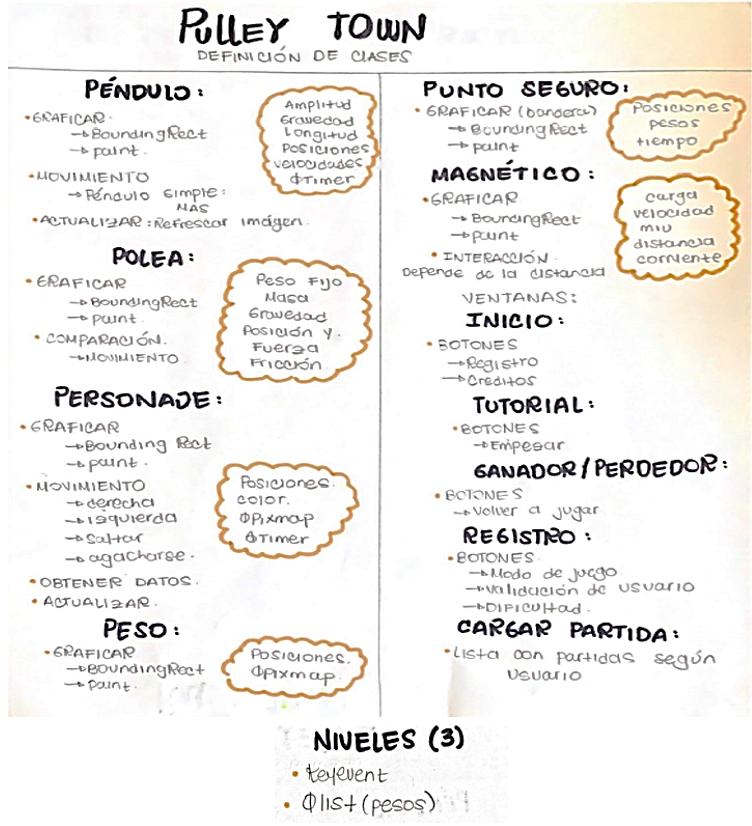
\includegraphics[scale=1]{diagrama1.PNG}
      \caption{Diagrama clases.}
      \label{fig:Diagrama}
   \end{figure}
\begin{itemize}
\item Péndulo: Se va a trabajar con un péndulo simple, el cual será uno de los obstáculos en los niveles.
\item Polea: Es el objetivo principal del juego, deberá verse si el peso que acumuló el jugador es suficiente para evitar que el peso fijo (según el nivel) llegue al piso.
\item Magnético: Se utilizará fuerza magnética como un obstáculo más, proveniente de un cable (Se comporta como un imán) el cual lleva una corriente. Para que la interacción magnética exista depende de la distancia, es decir existe una franja en la que el jugador será atraído por la fuerza magnética.
\item Personaje: El jugador podrá desplazarse hacia los lados, saltar y agacharse para lograr pasar por los obstáculos.
\item Punto-seguro: Son banderas que permitirán cargar partidas.
\item Niveles: Cada nivel tendrá diferentes tipos de superficies, es decir en algunas zonas existirá más o menos fricción y viscosidad.
\item Tanto el registro de usuarios, como la carga de partidas se desarrollarán por medio de archivos de texto.
\end{itemize}

\section{Cronograma:}
\begin{figure}[H]
      \centering
      \captionsetup{justification=centering}
      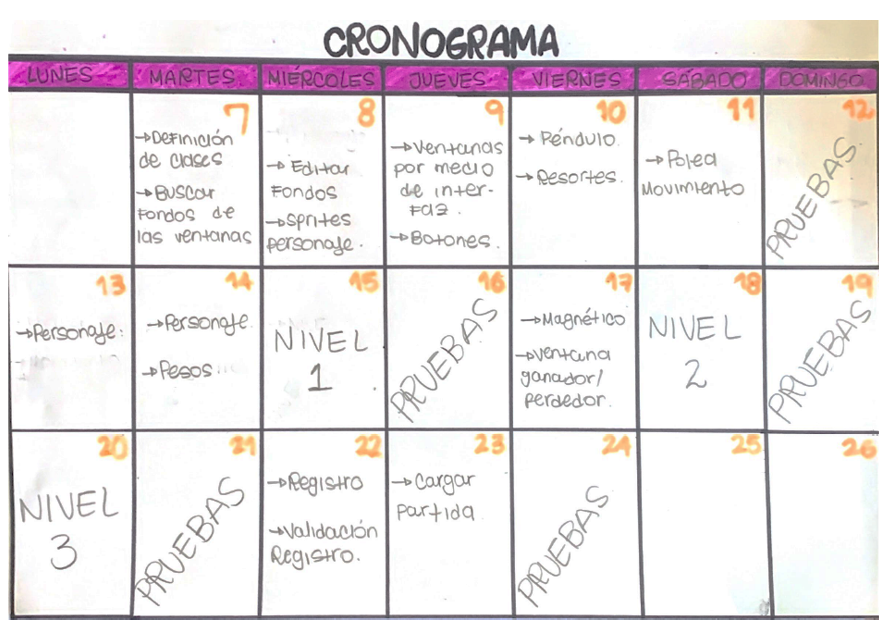
\includegraphics[scale=0.7]{crono.PNG}
      \caption{Cronograma.}
      \label{fig:Cronograma.}
   \end{figure}
\end{document}
